\section{Background}
\label{bg}

A brief overview on Linux asynchronous I/O ,NFS Ganesha and about callbacks will help us to understand the current system better.The asynchronous I/O stable version has been first introduced in Linux 2.6. A process that issues an Asynchronous I/O request doesn't have to wait for the availability of the data. Instead, after an I/O request is submitted, the process continues to execute its code and can later check the status of the submitted request. The Linux kernel exposes 5 system calls \cite{kernelCode} for supporting asynchronous I/O. We are listing them below with a brief description about each of them.

\begin{enumerate}

\item{\textbf{io\_setup()}: This system call is used to create an asynchronous I/O context in the kernel. Asynchronous I/O context is a set of data structures that the kernel provides to perform asynchronous I/O.}

\item{\textbf{io\_submit()}: This system call queues the I/O request blocks for processing in the asynchronous I/O context.}

\item{\textbf{io\_getevents()}: This system call is used to read the events from the completion queue of the asynchronous I/O context.}

\item{\textbf{io\_destroy()}: This system call is used to destroy the asynchronous I/O context.}

\item{\textbf{io\_cancel()}: This system call is used to cancel the asynchronous I/O operation previously submitted using io\_submit().}

\end{enumerate}

\begin{figure*}[htp]
\centering
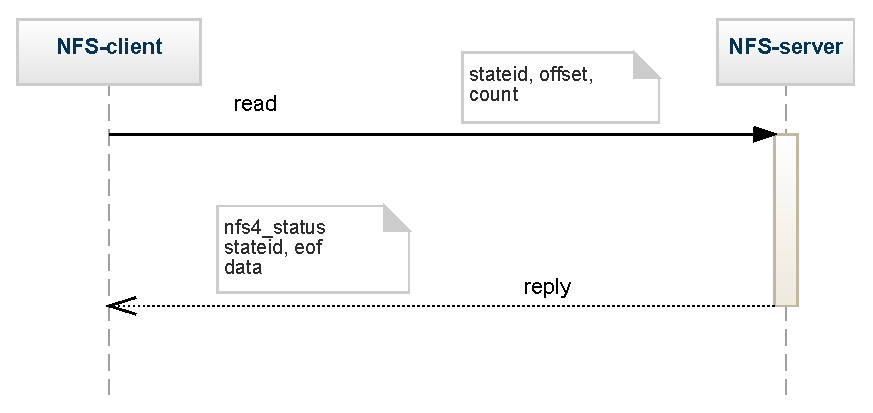
\includegraphics[scale=0.75]{figures/sequence_read.eps}
\caption{NFS Read Sequence Diagram}
\label{fig:NFSRead}
\end{figure*}

\begin{figure*}[htp]
\centering
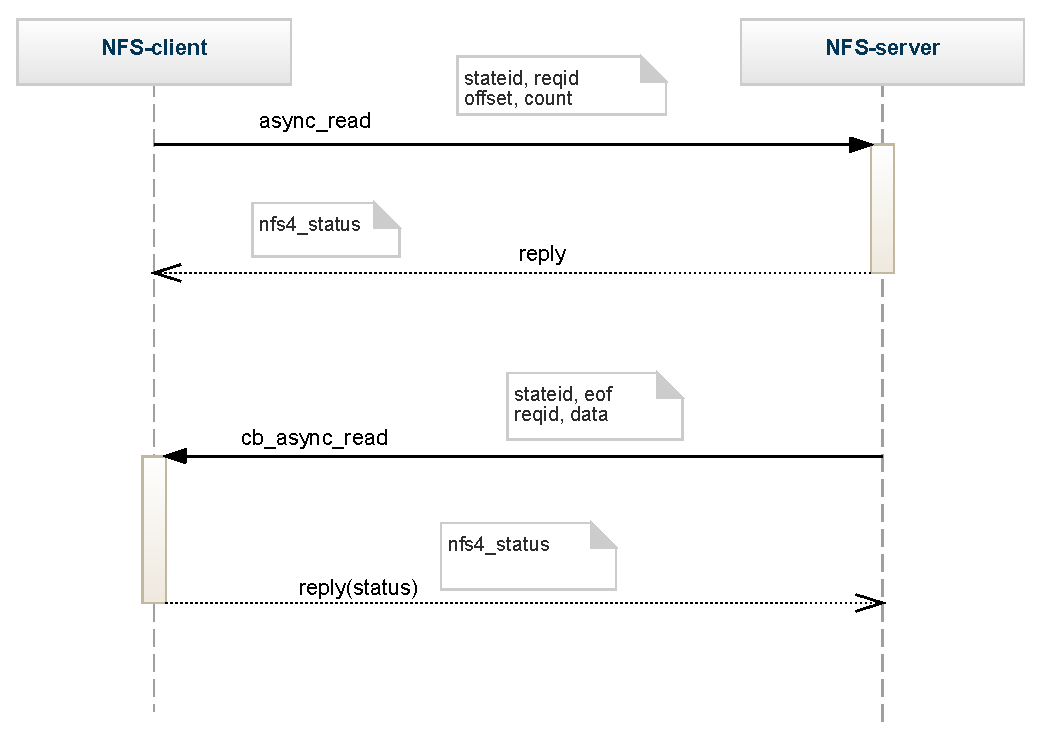
\includegraphics[scale=0.75]{figures/sequence_asyncread.eps}
\caption{NFS Asynchronous Read Sequence Diagram}
\label{fig:NFSAsyncRead}
\end{figure*}


Asynchronous I/O also works on NFS mounted files. But the underlying NFS stub initiates each of these requests and waits on the response synchronously. Using callbacks, these requests can be triggered concurrently. Callbacks provides a mechanism for the server to access the client. The client provides the server, its callback program number and port number using \textsc{setclientid}. The server does a backward path existence check before granting the delegation to the client. This check is done using \textsc{cb\_null} callback. The use of callbacks is not to be depended upon until the client has proven its ability to receive them. Thus in the implementation of the asynchronous I/O using callbacks, we need to follow the callback initiation steps, which include checking the existence of the backward path. If these checks do not succeed, the asynchronous I/O will fall back to the existing synchronous I/O mechanism. If the checks succeed, the server uses the callbacks to send data to the client.

   As we have mentioned in section 1 that NFS Ganesha is an user level implementation of NFS Server. It has a capability to serve multiple file systems at the same time. The other advantage of NFS Ganesha is, it manages huge meta-data cache. Because of this huge cache it can serve most of the nfs requests very fast. NFS Ganesha is built heavily on pthreads.
All the request processing is handled only by a pool of threads. The system performs better even in case of heavy loads as it has multiple threads to handle the load. Thus the system provide good guarantees on scalability. In Ganesha, the threads are classifies into two types, one is the dispatcher thread whose task is to decode incoming the nfs request and enqueue in the worker queue. The other type of threads are the worker threads whose task is to dequeue the request, process the request and return the reply to the corresponding client. In case of a error the worker thread will return the appropriate error.




%%%%%%%%%%%%%%%%%%%%%%%%%%%%%%%%%%%%%%%%%%%%%%%%%%%%%%%%%%%%%%%%%%%%%%%%%%%%%%
%% For Emacs:
% Local variables:
% fill-column: 70
% End:
%%%%%%%%%%%%%%%%%%%%%%%%%%%%%%%%%%%%%%%%%%%%%%%%%%%%%%%%%%%%%%%%%%%%%%%%%%%%%%
%% For Vim:
% vim:textwidth=70
%%%%%%%%%%%%%%%%%%%%%%%%%%%%%%%%%%%%%%%%%%%%%%%%%%%%%%%%%%%%%%%%%%%%%%%%%%%%%%
% LocalWords:  SMR HDDs drive's SMRs
